\documentclass[twoside]{book}

% Packages required by doxygen
\usepackage{fixltx2e}
\usepackage{calc}
\usepackage{doxygen}
\usepackage[export]{adjustbox} % also loads graphicx
\usepackage{graphicx}
\usepackage[utf8]{inputenc}
\usepackage{makeidx}
\usepackage{multicol}
\usepackage{multirow}
\PassOptionsToPackage{warn}{textcomp}
\usepackage{textcomp}
\usepackage[nointegrals]{wasysym}
\usepackage[table]{xcolor}

% Font selection
\usepackage[T1]{fontenc}
\usepackage[scaled=.90]{helvet}
\usepackage{courier}
\usepackage{amssymb}
\usepackage{sectsty}
\renewcommand{\familydefault}{\sfdefault}
\allsectionsfont{%
  \fontseries{bc}\selectfont%
  \color{darkgray}%
}
\renewcommand{\DoxyLabelFont}{%
  \fontseries{bc}\selectfont%
  \color{darkgray}%
}
\newcommand{\+}{\discretionary{\mbox{\scriptsize$\hookleftarrow$}}{}{}}

% Page & text layout
\usepackage{geometry}
\geometry{%
  a4paper,%
  top=2.5cm,%
  bottom=2.5cm,%
  left=2.5cm,%
  right=2.5cm%
}
\tolerance=750
\hfuzz=15pt
\hbadness=750
\setlength{\emergencystretch}{15pt}
\setlength{\parindent}{0cm}
\setlength{\parskip}{3ex plus 2ex minus 2ex}
\makeatletter
\renewcommand{\paragraph}{%
  \@startsection{paragraph}{4}{0ex}{-1.0ex}{1.0ex}{%
    \normalfont\normalsize\bfseries\SS@parafont%
  }%
}
\renewcommand{\subparagraph}{%
  \@startsection{subparagraph}{5}{0ex}{-1.0ex}{1.0ex}{%
    \normalfont\normalsize\bfseries\SS@subparafont%
  }%
}
\makeatother

% Headers & footers
\usepackage{fancyhdr}
\pagestyle{fancyplain}
\fancyhead[LE]{\fancyplain{}{\bfseries\thepage}}
\fancyhead[CE]{\fancyplain{}{}}
\fancyhead[RE]{\fancyplain{}{\bfseries\leftmark}}
\fancyhead[LO]{\fancyplain{}{\bfseries\rightmark}}
\fancyhead[CO]{\fancyplain{}{}}
\fancyhead[RO]{\fancyplain{}{\bfseries\thepage}}
\fancyfoot[LE]{\fancyplain{}{}}
\fancyfoot[CE]{\fancyplain{}{}}
\fancyfoot[RE]{\fancyplain{}{\bfseries\scriptsize Generated by Doxygen }}
\fancyfoot[LO]{\fancyplain{}{\bfseries\scriptsize Generated by Doxygen }}
\fancyfoot[CO]{\fancyplain{}{}}
\fancyfoot[RO]{\fancyplain{}{}}
\renewcommand{\footrulewidth}{0.4pt}
\renewcommand{\chaptermark}[1]{%
  \markboth{#1}{}%
}
\renewcommand{\sectionmark}[1]{%
  \markright{\thesection\ #1}%
}

% Indices & bibliography
\usepackage{natbib}
\usepackage[titles]{tocloft}
\setcounter{tocdepth}{3}
\setcounter{secnumdepth}{5}
\makeindex

% Hyperlinks (required, but should be loaded last)
\usepackage{ifpdf}
\ifpdf
  \usepackage[pdftex,pagebackref=true]{hyperref}
\else
  \usepackage[ps2pdf,pagebackref=true]{hyperref}
\fi
\hypersetup{%
  colorlinks=true,%
  linkcolor=blue,%
  citecolor=blue,%
  unicode%
}

% Custom commands
\newcommand{\clearemptydoublepage}{%
  \newpage{\pagestyle{empty}\cleardoublepage}%
}

\usepackage{caption}
\captionsetup{labelsep=space,justification=centering,font={bf},singlelinecheck=off,skip=4pt,position=top}

%===== C O N T E N T S =====

\begin{document}

% Titlepage & ToC
\hypersetup{pageanchor=false,
             bookmarksnumbered=true,
             pdfencoding=unicode
            }
\pagenumbering{alph}
\begin{titlepage}
\vspace*{7cm}
\begin{center}%
{\Large Frontaccounting Inventory Counting Module }\\
\vspace*{1cm}
{\large Generated by Doxygen 1.8.12}\\
\end{center}
\end{titlepage}
\clearemptydoublepage
\pagenumbering{roman}
\tableofcontents
\clearemptydoublepage
\pagenumbering{arabic}
\hypersetup{pageanchor=true}

%--- Begin generated contents ---
\chapter{Hierarchical Index}
\section{Class Hierarchy}
This inheritance list is sorted roughly, but not completely, alphabetically\+:\begin{DoxyCompactList}
\item generic\+\_\+fa\+\_\+interface\begin{DoxyCompactList}
\item \contentsline{section}{ksf\+\_\+qoh}{\pageref{classksf__qoh}}{}
\end{DoxyCompactList}
\item hooks\begin{DoxyCompactList}
\item \contentsline{section}{hooks\+\_\+ksf\+\_\+qoh}{\pageref{classhooks__ksf__qoh}}{}
\end{DoxyCompactList}
\end{DoxyCompactList}

\chapter{Class Index}
\section{Class List}
Here are the classes, structs, unions and interfaces with brief descriptions\+:\begin{DoxyCompactList}
\item\contentsline{section}{\hyperlink{classgeneric__interface}{generic\+\_\+interface} }{\pageref{classgeneric__interface}}{}
\item\contentsline{section}{\hyperlink{classgeneric__orders}{generic\+\_\+orders} }{\pageref{classgeneric__orders}}{}
\item\contentsline{section}{\hyperlink{classhooks___inventory}{hooks\+\_\+\+Inventory} }{\pageref{classhooks___inventory}}{}
\item\contentsline{section}{\hyperlink{class_inventory}{Inventory} }{\pageref{class_inventory}}{}
\item\contentsline{section}{\hyperlink{classinventory__cart}{inventory\+\_\+cart} }{\pageref{classinventory__cart}}{}
\item\contentsline{section}{\hyperlink{class_inventory__ui}{Inventory\+\_\+ui} }{\pageref{class_inventory__ui}}{}
\item\contentsline{section}{\hyperlink{classitem}{item} }{\pageref{classitem}}{}
\end{DoxyCompactList}

\chapter{Class Documentation}
\hypertarget{classgeneric__orders}{}\section{generic\+\_\+orders Class Reference}
\label{classgeneric__orders}\index{generic\+\_\+orders@{generic\+\_\+orders}}
Inheritance diagram for generic\+\_\+orders\+:\begin{figure}[H]
\begin{center}
\leavevmode
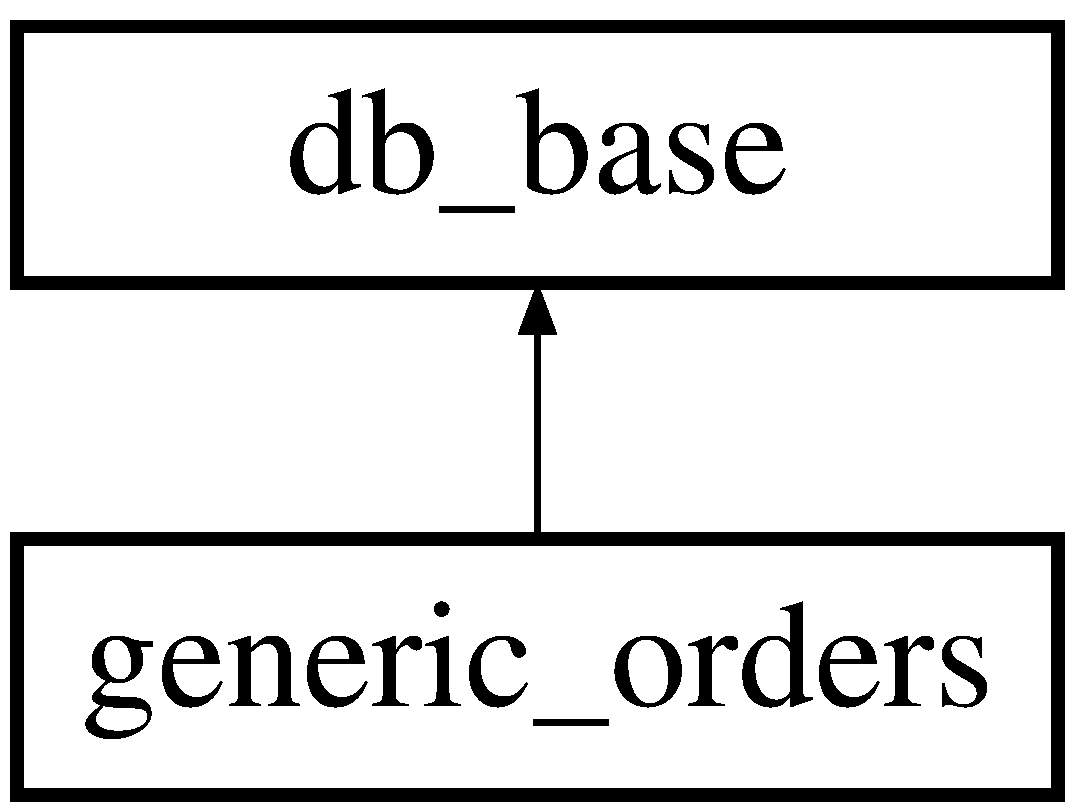
\includegraphics[height=2.000000cm]{d3/d2b/classgeneric__orders}
\end{center}
\end{figure}
\subsection*{Public Member Functions}
\begin{DoxyCompactItemize}
\item 
\hypertarget{classgeneric__orders_ad96a6adbcf3f1d2eaec7b3eefcf8cb8c}{}\label{classgeneric__orders_ad96a6adbcf3f1d2eaec7b3eefcf8cb8c} 
{\bfseries \+\_\+\+\_\+construct} ( \$host, \$user, \$pass, \$database, \$pref\+\_\+tablename)
\item 
\hypertarget{classgeneric__orders_a73da33c51344d619ad219c5c3533157a}{}\label{classgeneric__orders_a73da33c51344d619ad219c5c3533157a} 
{\bfseries install} ()
\item 
\hypertarget{classgeneric__orders_ac0a1f57dd5fe0ee9cad423a8581323b9}{}\label{classgeneric__orders_ac0a1f57dd5fe0ee9cad423a8581323b9} 
{\bfseries get\+\_\+purchase\+\_\+order} ()
\item 
\hypertarget{classgeneric__orders_a636930f29dd1a4214d9beb7b0b992fb2}{}\label{classgeneric__orders_a636930f29dd1a4214d9beb7b0b992fb2} 
{\bfseries get\+\_\+id\+\_\+range} ()
\item 
\hypertarget{classgeneric__orders_a77d76b233e40d4c76e7d93c4a2b87815}{}\label{classgeneric__orders_a77d76b233e40d4c76e7d93c4a2b87815} 
{\bfseries get\+\_\+supplier\+\_\+order} ()
\item 
\hypertarget{classgeneric__orders_afb2ea2f9acc44492b9f1880f31131df5}{}\label{classgeneric__orders_afb2ea2f9acc44492b9f1880f31131df5} 
{\bfseries export\+\_\+orders} ()
\item 
\hypertarget{classgeneric__orders_a5921f90917717297983148c16bfcdff7}{}\label{classgeneric__orders_a5921f90917717297983148c16bfcdff7} 
{\bfseries loadprefs} ()
\item 
\hypertarget{classgeneric__orders_a713ac2d657b69a5b68bcd93c085f6bff}{}\label{classgeneric__orders_a713ac2d657b69a5b68bcd93c085f6bff} 
{\bfseries updateprefs} ()
\item 
\hypertarget{classgeneric__orders_a733f9e1d53da1f2002ad5580d6215baf}{}\label{classgeneric__orders_a733f9e1d53da1f2002ad5580d6215baf} 
{\bfseries checkprefs} ()
\item 
\hypertarget{classgeneric__orders_a58246a65d39b0a1f79a520c54bf160a5}{}\label{classgeneric__orders_a58246a65d39b0a1f79a520c54bf160a5} 
{\bfseries action\+\_\+show\+\_\+form} ()
\item 
\hypertarget{classgeneric__orders_ae17ab2370a928c300c4900d1b14976d2}{}\label{classgeneric__orders_ae17ab2370a928c300c4900d1b14976d2} 
{\bfseries form\+\_\+export} ()
\item 
\hypertarget{classgeneric__orders_a9510fade9bbc4e505930f08750ef1c5f}{}\label{classgeneric__orders_a9510fade9bbc4e505930f08750ef1c5f} 
{\bfseries related\+\_\+tabs} ()
\item 
\hypertarget{classgeneric__orders_a04c2ba96918f5aed83649677feec28d5}{}\label{classgeneric__orders_a04c2ba96918f5aed83649677feec28d5} 
{\bfseries show\+\_\+form} ()
\item 
\hypertarget{classgeneric__orders_adda352a9a97d7d94b34e2ad5289643d2}{}\label{classgeneric__orders_adda352a9a97d7d94b34e2ad5289643d2} 
{\bfseries base\+\_\+page} ()
\item 
\hypertarget{classgeneric__orders_a30d91bc07b565db854032cf4687583b6}{}\label{classgeneric__orders_a30d91bc07b565db854032cf4687583b6} 
{\bfseries display} ()
\item 
\hypertarget{classgeneric__orders_aa26ae7d2601973a71a16a0f40a9946f8}{}\label{classgeneric__orders_aa26ae7d2601973a71a16a0f40a9946f8} 
{\bfseries run} ()
\end{DoxyCompactItemize}
\subsection*{Public Attributes}
\begin{DoxyCompactItemize}
\item 
\hypertarget{classgeneric__orders_a9a99b3d242d00f9dff29c452930cdc46}{}\label{classgeneric__orders_a9a99b3d242d00f9dff29c452930cdc46} 
{\bfseries \$order\+\_\+no}
\item 
\hypertarget{classgeneric__orders_a5b9ac946cce6674e2b7abcfd396f82ea}{}\label{classgeneric__orders_a5b9ac946cce6674e2b7abcfd396f82ea} 
{\bfseries \$db\+\_\+\+Host}
\item 
\hypertarget{classgeneric__orders_a24279845da685a00cf035df4bbe339d1}{}\label{classgeneric__orders_a24279845da685a00cf035df4bbe339d1} 
{\bfseries \$db\+\_\+\+User}
\item 
\hypertarget{classgeneric__orders_af6abeff7193a46c1785edef999aebe72}{}\label{classgeneric__orders_af6abeff7193a46c1785edef999aebe72} 
{\bfseries \$db\+\_\+\+Password}
\item 
\hypertarget{classgeneric__orders_ab37c01fb6bfad57f908e01b6c65e5d9d}{}\label{classgeneric__orders_ab37c01fb6bfad57f908e01b6c65e5d9d} 
{\bfseries \$db\+\_\+\+Name}
\item 
\hypertarget{classgeneric__orders_a723c673ed302846be920efe7ef6b656e}{}\label{classgeneric__orders_a723c673ed302846be920efe7ef6b656e} 
{\bfseries \$last\+\_\+order\+\_\+no}
\item 
\hypertarget{classgeneric__orders_a9eb2c59dd61c0dde32ff3171a522bd69}{}\label{classgeneric__orders_a9eb2c59dd61c0dde32ff3171a522bd69} 
{\bfseries \$vendor}
\item 
\hypertarget{classgeneric__orders_ae9ac8a364ccd57159c7c2f7cb9828444}{}\label{classgeneric__orders_ae9ac8a364ccd57159c7c2f7cb9828444} 
{\bfseries \$tabs} = array()
\item 
\hypertarget{classgeneric__orders_a8b5bbce48d66545ab58b43f4be772872}{}\label{classgeneric__orders_a8b5bbce48d66545ab58b43f4be772872} 
{\bfseries \$found}
\item 
\hypertarget{classgeneric__orders_ad9f0450540b7abed0a3952217421268b}{}\label{classgeneric__orders_ad9f0450540b7abed0a3952217421268b} 
{\bfseries \$purchase\+\_\+order}
\item 
\hypertarget{classgeneric__orders_aa9882dc26f8860b93d947905dfca7483}{}\label{classgeneric__orders_aa9882dc26f8860b93d947905dfca7483} 
{\bfseries \$config\+\_\+values} = array()
\item 
\hypertarget{classgeneric__orders_a0886ded57343072f2ad3821288d00454}{}\label{classgeneric__orders_a0886ded57343072f2ad3821288d00454} 
{\bfseries \$help\+\_\+context}
\item 
\hypertarget{classgeneric__orders_acfdc001bf2e21ac8d63d8265f3b2dd3f}{}\label{classgeneric__orders_acfdc001bf2e21ac8d63d8265f3b2dd3f} 
{\bfseries \$action}
\item 
\hypertarget{classgeneric__orders_ad884a4bee50042666a9c9aebece716bd}{}\label{classgeneric__orders_ad884a4bee50042666a9c9aebece716bd} 
{\bfseries \$redirect\+\_\+to}
\end{DoxyCompactItemize}


The documentation for this class was generated from the following file\+:\begin{DoxyCompactItemize}
\item 
class.\+generic\+\_\+orders.\+php\end{DoxyCompactItemize}

\hypertarget{classhooks__ksf__generate__catalogue}{}\section{hooks\+\_\+ksf\+\_\+generate\+\_\+catalogue Class Reference}
\label{classhooks__ksf__generate__catalogue}\index{hooks\+\_\+ksf\+\_\+generate\+\_\+catalogue@{hooks\+\_\+ksf\+\_\+generate\+\_\+catalogue}}
Inheritance diagram for hooks\+\_\+ksf\+\_\+generate\+\_\+catalogue\+:\begin{figure}[H]
\begin{center}
\leavevmode
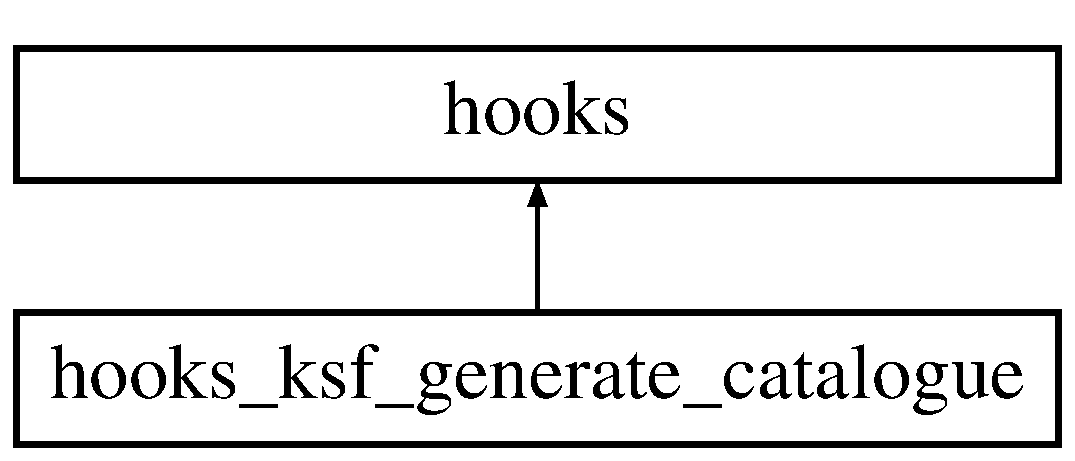
\includegraphics[height=2.000000cm]{dd/d8c/classhooks__ksf__generate__catalogue}
\end{center}
\end{figure}
\subsection*{Public Member Functions}
\begin{DoxyCompactItemize}
\item 
\hypertarget{classhooks__ksf__generate__catalogue_ac4dd1b1aa750811bb9b32dc195fcf420}{}\label{classhooks__ksf__generate__catalogue_ac4dd1b1aa750811bb9b32dc195fcf420} 
{\bfseries install\+\_\+options} (\$app)
\item 
\hypertarget{classhooks__ksf__generate__catalogue_ae15273e8ca8ceb7f37bdddc3211776d6}{}\label{classhooks__ksf__generate__catalogue_ae15273e8ca8ceb7f37bdddc3211776d6} 
{\bfseries install\+\_\+access} ()
\end{DoxyCompactItemize}
\subsection*{Public Attributes}
\begin{DoxyCompactItemize}
\item 
\hypertarget{classhooks__ksf__generate__catalogue_a9847dd3a50ee2ee5c2c77297514663b7}{}\label{classhooks__ksf__generate__catalogue_a9847dd3a50ee2ee5c2c77297514663b7} 
{\bfseries \$module\+\_\+name} = \textquotesingle{}Generate Catalogue\textquotesingle{}
\end{DoxyCompactItemize}


The documentation for this class was generated from the following file\+:\begin{DoxyCompactItemize}
\item 
hooks.\+php\end{DoxyCompactItemize}

\hypertarget{classksf__generate__catalogue}{}\section{ksf\+\_\+generate\+\_\+catalogue Class Reference}
\label{classksf__generate__catalogue}\index{ksf\+\_\+generate\+\_\+catalogue@{ksf\+\_\+generate\+\_\+catalogue}}
Inheritance diagram for ksf\+\_\+generate\+\_\+catalogue\+:\begin{figure}[H]
\begin{center}
\leavevmode
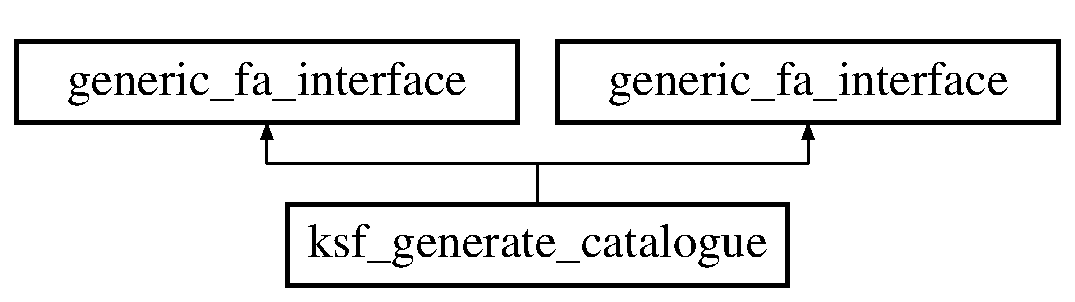
\includegraphics[height=2.000000cm]{d1/dec/classksf__generate__catalogue}
\end{center}
\end{figure}
\subsection*{Public Member Functions}
\begin{DoxyCompactItemize}
\item 
\hypertarget{classksf__generate__catalogue_a62c6426c5da97539abe147da4858ddee}{}\label{classksf__generate__catalogue_a62c6426c5da97539abe147da4858ddee} 
{\bfseries \+\_\+\+\_\+construct} ( \$pref\+\_\+tablename)
\item 
\hypertarget{classksf__generate__catalogue_a62c6426c5da97539abe147da4858ddee}{}\label{classksf__generate__catalogue_a62c6426c5da97539abe147da4858ddee} 
{\bfseries \+\_\+\+\_\+construct} ( \$pref\+\_\+tablename)
\item 
\hypertarget{classksf__generate__catalogue_a4a992db7cec6b25c91ed4a7f442fd7d4}{}\label{classksf__generate__catalogue_a4a992db7cec6b25c91ed4a7f442fd7d4} 
{\bfseries prep\+\_\+write\+\_\+file} ()
\item 
\hypertarget{classksf__generate__catalogue_a64728d4da61510a9a3acb5953fa0bfdc}{}\label{classksf__generate__catalogue_a64728d4da61510a9a3acb5953fa0bfdc} 
{\bfseries create\+\_\+price\+\_\+book} ()
\item 
\hypertarget{classksf__generate__catalogue_a727667dd018f1855cddae13cba43e89d}{}\label{classksf__generate__catalogue_a727667dd018f1855cddae13cba43e89d} 
{\bfseries create\+\_\+sku\+\_\+labels} ()
\item 
\hyperlink{classksf__generate__catalogue_a4a0e6c124aeb3ecc1078183b462f74d2}{create\+\_\+sku\+\_\+labels\+\_\+from\+\_\+\+PO} ()
\item 
\hypertarget{classksf__generate__catalogue_a94e7cc96f637746a840ba8c887f26338}{}\label{classksf__generate__catalogue_a94e7cc96f637746a840ba8c887f26338} 
{\bfseries email\+\_\+price\+\_\+book} ()
\item 
\hypertarget{classksf__generate__catalogue_a9b66cc71e9240a3a1e6dfdb980bc6c8d}{}\label{classksf__generate__catalogue_a9b66cc71e9240a3a1e6dfdb980bc6c8d} 
{\bfseries form\+\_\+pricebook} ()
\item 
\hypertarget{classksf__generate__catalogue_adb6450984931cd24cfc6b21cdc9ec30e}{}\label{classksf__generate__catalogue_adb6450984931cd24cfc6b21cdc9ec30e} 
{\bfseries write\+\_\+file\+\_\+form} ()
\item 
\hypertarget{classksf__generate__catalogue_a0680dd5373558234df5ec3e6ba492b8a}{}\label{classksf__generate__catalogue_a0680dd5373558234df5ec3e6ba492b8a} 
{\bfseries polabelsfile\+\_\+form} ()
\item 
\hypertarget{classksf__generate__catalogue_ad9f7b9e3916d0171cac9c28e95a2e20a}{}\label{classksf__generate__catalogue_ad9f7b9e3916d0171cac9c28e95a2e20a} 
{\bfseries label\+\_\+export} ()
\item 
\hyperlink{classksf__generate__catalogue_a23e86ab2d815a549d625fcf34df36003}{label\+\_\+export\+\_\+by\+\_\+\+P\+O\+\_\+\+Delivery} ()
\end{DoxyCompactItemize}
\subsection*{Public Attributes}
\begin{DoxyCompactItemize}
\item 
\hypertarget{classksf__generate__catalogue_a612505b2b69c7d3ed108ac2e54757b65}{}\label{classksf__generate__catalogue_a612505b2b69c7d3ed108ac2e54757b65} 
\hyperlink{classksf__generate__catalogue_a612505b2b69c7d3ed108ac2e54757b65}{\$write\+\_\+file}
\begin{DoxyCompactList}\small\item\em class write\+\_\+file for writing files \end{DoxyCompactList}\item 
\hypertarget{classksf__generate__catalogue_a0763eb90512a79279547aed50be5af0e}{}\label{classksf__generate__catalogue_a0763eb90512a79279547aed50be5af0e} 
{\bfseries \$include\+\_\+header}
\item 
\hypertarget{classksf__generate__catalogue_a0752ca8313f8601730b2873dd2565709}{}\label{classksf__generate__catalogue_a0752ca8313f8601730b2873dd2565709} 
{\bfseries \$maxrowsallowed}
\item 
\hypertarget{classksf__generate__catalogue_a16a2169010e4f6d91ca9bd9858503dd3}{}\label{classksf__generate__catalogue_a16a2169010e4f6d91ca9bd9858503dd3} 
{\bfseries \$lastoid}
\item 
\hypertarget{classksf__generate__catalogue_a0228d54fbc983f9e657b2f26e6f823cc}{}\label{classksf__generate__catalogue_a0228d54fbc983f9e657b2f26e6f823cc} 
{\bfseries \$mailto}
\item 
\hypertarget{classksf__generate__catalogue_af493b5c8338346fa2bb17832abfba18b}{}\label{classksf__generate__catalogue_af493b5c8338346fa2bb17832abfba18b} 
{\bfseries \$mailfrom}
\item 
\hypertarget{classksf__generate__catalogue_af6e3f59fbde0869fedda9ced3b473766}{}\label{classksf__generate__catalogue_af6e3f59fbde0869fedda9ced3b473766} 
{\bfseries \$db}
\item 
\hypertarget{classksf__generate__catalogue_a162951a4881323934a3354795a92a3df}{}\label{classksf__generate__catalogue_a162951a4881323934a3354795a92a3df} 
{\bfseries \$environment}
\item 
\hypertarget{classksf__generate__catalogue_a0e69b1864f0d52d5d28c1eed69e8c19b}{}\label{classksf__generate__catalogue_a0e69b1864f0d52d5d28c1eed69e8c19b} 
{\bfseries \$maxpics}
\item 
\hypertarget{classksf__generate__catalogue_a7db85ede795314de6395a5644f3423b7}{}\label{classksf__generate__catalogue_a7db85ede795314de6395a5644f3423b7} 
{\bfseries \$debug}
\item 
\hypertarget{classksf__generate__catalogue_ae71f41906b583edc52da3bbda5136a2c}{}\label{classksf__generate__catalogue_ae71f41906b583edc52da3bbda5136a2c} 
{\bfseries \$fields\+\_\+array}
\item 
\hypertarget{classksf__generate__catalogue_a5690da45df838f429077df5bf5a95563}{}\label{classksf__generate__catalogue_a5690da45df838f429077df5bf5a95563} 
{\bfseries \$dolabels}
\end{DoxyCompactItemize}


\subsection{Detailed Description}
uses inherited call\+\_\+table uses class write\+\_\+file uses class email\+\_\+file 

\subsection{Member Function Documentation}
\hypertarget{classksf__generate__catalogue_a4a0e6c124aeb3ecc1078183b462f74d2}{}\label{classksf__generate__catalogue_a4a0e6c124aeb3ecc1078183b462f74d2} 
\index{ksf\+\_\+generate\+\_\+catalogue@{ksf\+\_\+generate\+\_\+catalogue}!create\+\_\+sku\+\_\+labels\+\_\+from\+\_\+\+PO@{create\+\_\+sku\+\_\+labels\+\_\+from\+\_\+\+PO}}
\index{create\+\_\+sku\+\_\+labels\+\_\+from\+\_\+\+PO@{create\+\_\+sku\+\_\+labels\+\_\+from\+\_\+\+PO}!ksf\+\_\+generate\+\_\+catalogue@{ksf\+\_\+generate\+\_\+catalogue}}
\subsubsection{\texorpdfstring{create\+\_\+sku\+\_\+labels\+\_\+from\+\_\+\+P\+O()}{create\_sku\_labels\_from\_PO()}}
{\footnotesize\ttfamily ksf\+\_\+generate\+\_\+catalogue\+::create\+\_\+sku\+\_\+labels\+\_\+from\+\_\+\+PO (\begin{DoxyParamCaption}{ }\end{DoxyParamCaption})}

Generate labels from a purchase order \hypertarget{classksf__generate__catalogue_a23e86ab2d815a549d625fcf34df36003}{}\label{classksf__generate__catalogue_a23e86ab2d815a549d625fcf34df36003} 
\index{ksf\+\_\+generate\+\_\+catalogue@{ksf\+\_\+generate\+\_\+catalogue}!label\+\_\+export\+\_\+by\+\_\+\+P\+O\+\_\+\+Delivery@{label\+\_\+export\+\_\+by\+\_\+\+P\+O\+\_\+\+Delivery}}
\index{label\+\_\+export\+\_\+by\+\_\+\+P\+O\+\_\+\+Delivery@{label\+\_\+export\+\_\+by\+\_\+\+P\+O\+\_\+\+Delivery}!ksf\+\_\+generate\+\_\+catalogue@{ksf\+\_\+generate\+\_\+catalogue}}
\subsubsection{\texorpdfstring{label\+\_\+export\+\_\+by\+\_\+\+P\+O\+\_\+\+Delivery()}{label\_export\_by\_PO\_Delivery()}}
{\footnotesize\ttfamily ksf\+\_\+generate\+\_\+catalogue\+::label\+\_\+export\+\_\+by\+\_\+\+P\+O\+\_\+\+Delivery (\begin{DoxyParamCaption}{ }\end{DoxyParamCaption})}

Given a PO number create the labels for the items in that PO

\begin{DoxyReturn}{Returns}
bool 
\end{DoxyReturn}


The documentation for this class was generated from the following files\+:\begin{DoxyCompactItemize}
\item 
class.\+ksf\+\_\+generate\+\_\+catalogue.\+min.\+php\item 
class.\+ksf\+\_\+generate\+\_\+catalogue.\+php\end{DoxyCompactItemize}

%--- End generated contents ---

% Index
\backmatter
\newpage
\phantomsection
\clearemptydoublepage
\addcontentsline{toc}{chapter}{Index}
\printindex

\end{document}
